\cotefile{136}
\scanpage{364}
\mspage{3}
\diagram{\begin{tikzcd}[row sep=large]
\underline{H_*(K(\mathbb F_p,n),\mathbb F_p)}^*\simeq H^{n+r}(K(\mathbb F_p,n),\mathbb F_p)\arrow[d,bend left=15]\\
\text{operations coh de type}
\end{tikzcd}}
\diagram{\begin{tikzcd}
K(Z,n)\arrow[r]&K(Z,n\arrow[r]&K(\mathbb F_p,n)
\end{tikzcd}}
Puisque $K(\mathbb F_p,n)$ représente la $\mathbb F_p$, coh
\[
(\mathbb F_p,n,\mathbb F_p,n+r)
\]
$r<n$

Operations stables de deg $r$

$\{P_r\}$\qquad Une collection $\forall n$
\diagram{\begin{tikzcd}
H^n(X,\mathbb F_p)\arrow[r]&H^{n+r}(X,\mathbb F_p)
\end{tikzcd}}
commute
\diagram{\begin{tikzcd}[column sep=large]
\overline H^{n+1}(SX,\mathbb F_p)\arrow[r,"P_{n+1}"]\arrow[d,draw=none,"{\rotatebox{90}{$\simeq$}}" description]&\overline H^{n+1+r}(SX,\mathbb F_p)\arrow[d,draw=none,"{\rotatebox{90}{$\simeq$}}" description]\\
\widetilde H^n(X,\mathbb F_p)\arrow[r,"P_n"]&\widetilde H^{n+r}(X,\mathbb F_p)
\end{tikzcd}}
\margin{$r<n$}
\diagram{\begin{tikzcd}[column sep=small]
&H^{n+r}(K(\mathbb F_p,n),\mathbb F_p)\arrow[dl]&\simeq H^{n+r+1}(K(\mathbb F_p,n+1),\mathbb F_p)\\
H^{n+r-1}(K(\mathbb F_p,n-1,\mathbb F_p)&P_n'&P_{n+1}'
\end{tikzcd}}

\uuline{Operations stables}: Les op stable sont \deleted{\unsure{el}} donnés par l'algebre de Steenrod

$p\ne2$
\[
\mathbb F_p[\underline{P^0,P^1,\ldots P^n,\ldots,\beta}]
\]
\[
P^0=1\qquad\deg P^i=2i(p-1)\qquad\deg\beta=1
\]
Relations d'Adem

\margin{Cohomology operations\par
Steenrod $+$ Epstein\par
Ann of Math Studies N° 50\par
Princeton\par
p 77}
\mspage{365}

\scanpage{365}
$P^i$ op stables construite par Steenrod.
\mspage{4}

$p=2$
\[
\mathbb F_2\underline{[\operatorname{Sq}^i]}\qquad i\geq0
\]
\[
\operatorname{Sq}^0=1\qquad(\operatorname{Sq}^1=\beta)\quad\text{rel d'Adem}
\]
$\deg\operatorname{Sq}^i=i$

\margin{$p\quad2$}
\deleted{$\operatorname{Sq}^1\operatorname{Sq}^2=\operatorname{Sq}$}
\[
\operatorname{Sq}^1\operatorname{Sq}^2=\operatorname{Sq}^3+\operatorname{Sq}^2\operatorname{Sq}^1\qquad(?)
\]
etc --
\figure{\begin{tikzpicture}\draw (0,0) .. controls (.4,.02) and (.6,0) .. (.8,-.02);\end{tikzpicture}}

Formule de Cartan:
\[
P^i(x\times y)=\sum_{j\geq0}P^j(x)P^{i-j}(y)
\]
\[
P^I=\beta^{\epsilon_0}P^{\eta_1}\beta^{\epsilon_1}P^{\eta_2}\ldots
\qquad\mathord{\begin{tikzpicture}[baseline=(I.base)]\node[draw,ellipse,inner sep=2pt] (I) {$I$};\end{tikzpicture}}\sim(\epsilon_0,\eta_1,\epsilon_1,\eta_2,\ldots)
\]
\margin{deg $I$ de maniere evidente\par
excès $e(I)=\text{``}\eta_1-\sum_{i>1}\eta_i\text{''}$}
\[
\epsilon_i=0,1\qquad\eta_i\geq0
\]
admissible
\[
\eta_i\geq p\eta_{i+1}+\epsilon_i
\]
les $P^I$ admissible forment une $\mathbb F_p$ base.
\figure{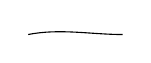
\begin{tikzpicture}\draw (0,0) .. controls (.4,.08) and (.8,0) .. (1.2,0);\end{tikzpicture}}
\diagram{\begin{tikzcd}[column sep=large]
|[draw,ellipse]| A\arrow[r]&H^*(K(\mathbb F_p,n),\mathbb F_p)\\
x&|[draw,ellipse]| x\iota_n
\end{tikzcd}}

\uline{Theoréme}.
\margin{Serre ($p=2$)}
\[
H^*(K(\mathbb F_p,n),\mathbb F_p)=
\]
Algebre anticommutative libre sur $\mathbb F_p$ engendrée par le \uline{monomes admissibles} d'exces $<n$.
\[
H_*(\underline{K(\mathbb F_p,n)},\mathbb F_p)=
\]
Alg anticom à puiss divisée universelle engendrée par le elements duaux.
\mspage{366}

\scanpage{366}
\mspage{5}
\uline{Dem 1)}\quad Seminaire Cartan

On regarde la suite spectrale du classifiant
\[
E_2\simeq\operatorname{Tor}^{H_*(K(\mathbb F_p,n),\mathbb F_p)}(\mathbb F_p,\mathbb F_p)
\Longrightarrow H_*(\underbrace{K(\mathbb F_p,n+1),\mathbb F_p}_{\substack{\rotatebox{90}{$=$}\\\mathord{\begin{tikzpicture}[baseline=(B.base)]\node[draw,ellipse,inner sep=2pt] (B) {$B_{K(\mathbb F_p,n)}$};\end{tikzpicture}}}}]
\]
Suite sp d'Eilenberg - Moore

Steenrod - Rothenberger, etc --
\figure{\begin{tikzpicture}
\draw (0,.8)--(.15,.82);\draw (.35,.75)--(.8,.76);\draw (1.05,.72)--(1.5,.7);\draw (1.5,.7)--(1.58,.59);\draw (1.85,.65)--(2,.65);\draw (2.45,.52)--(2.5,.54);
\draw (-.4,-.5)--(0,-.1)--(.1,-.14)--(1.1,-.02);\draw (2.1,.02) .. controls (2.35,.02) and (2.4,-.08) .. (2.5,-.08);
\end{tikzpicture}}
\diagram{\begin{tikzcd}[column sep=small]
\underline{Z(G\times G)}&\mathord{\begin{tikzpicture}[baseline=(ZG.base)]\node[draw,ellipse,inner sep=2pt] (ZG) {$ZG$};\draw (ZG.center) ellipse (0.45 and 0.30);\draw (ZG.center) ellipse (0.52 and 0.37);\end{tikzpicture}}\arrow[r]&\mathbb Z\\
ZG\otimes ZG\arrow[ur,shift left=3]\arrow[ur]\arrow[ur,shift right=3]&&{}
\end{tikzcd}}
\deleted{$\otimes ZK(\mathbb F_p,n)$}
\diagram{\begin{tikzcd}[column sep=small]
&&N\mathord{\begin{tikzpicture}[baseline=(ZK.base)]\node[draw,ellipse,inner sep=2pt] (ZK) {$\underline{\underline{ZK(\mathbb F_p,n)}}$};\end{tikzpicture}}&\simeq M\\
&&\text{alg diff graduée}&{}\\
&&\text{Bar Constr}\quad\text{augmentée.}\arrow[d,no head]&{}\\
\deleted{\otimes}H_*(K(\mathbb F_p,n)^{\otimes2}\arrow[r,shift left=3]\arrow[r]\arrow[r,shift right=3]&H_*K(\mathbb F_p,n)\arrow[r]&M_\bullet&{}
\end{tikzcd}}
\figure{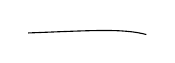
\begin{tikzpicture}\draw (0,0) .. controls (.8,.03) and (1.2,.06) .. (1.5,-.02);\end{tikzpicture}}
\[
A=Z(G)\qquad Z(EG)=*
\]
\diagram{\begin{tikzcd}[execute at end picture={\draw (0,0) ellipse (.7 and .3);\draw (0,0) ellipse (.8 and .35);}]
Z(BG)
\end{tikzcd}}
\figure{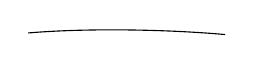
\begin{tikzpicture}\draw (0,0) .. controls (.7,.06) and (1.7,.05) .. (2.5,-.02);\end{tikzpicture}}

2) Methode de Serre\qquad Comm Helv\qquad1954
\margin{Springer:\par Symposium en l'honneur de Steenrod\par\uline{Article de}\par May.}
\[
H^*(K(\mathbb F,n+1,)\mathbb F_p)\otimes\underline{H^*(K(\mathbb F_p,n),\mathbb F_p)}\Longrightarrow\underline{H^*(*)}
\]
\figure{\begin{tikzpicture}\draw (0,.35) .. controls (-.35,.7) and (-.55,-.2) .. (0,-.3) .. controls (2,-.7) and (4,-.4) .. (4.5,-.1);\fill (.65,-.3) circle (.015);\fill (.8,-.4) circle (.015);\end{tikzpicture}}
\mspage{367}

\scanpage{367}
Comult naturelle sur $A$

$P$ operation coh
\[
(\mu^*P)(xy)=\sum P_i x\cdot P_j y
\]
Par la formule de Cartan
\[
\Delta P^i=\sum_{j+k=i}P^j\otimes P^k.
\]
\uline{Milnor}:
\[
\begin{array}{lll}
j\geq1&\xi_{\textcircled{\(j\)}}&\text{dual de }\underbrace{P^{p^{j-1}}\ldots P^{p^2}P^pP^{p^0}}_{\text{monome adm}}\\[1em]
j\geq0&\tau_j&P^{p^j}\ldots P^pP\beta
\end{array}
\]
\deleted{$\unsure{K(\mathbb F_p)}$}
\[
A_*=\operatorname{Sym}(\xi_i)\otimes\Lambda(\tau_{\deleted{k}j})
\]
dual de $A$

\[
L\operatorname{Sym}^r=0\qquad r\ne p^s\qquad s\geq0
\]
\[
L\operatorname{Sym}^{p^s}\deleted{K(\mathbb F_p,n)}
\]
\diagram{\begin{tikzcd}[column sep=large]
L_{n+i}\operatorname{Sym}K(\mathbb F_p,n)\arrow[r,"\substack{s\\+1}"]&L_{n+i+1}\operatorname{Sym}K(\mathbb F_p,n+1)
\end{tikzcd}}
\diagram{\begin{tikzcd}[column sep=0pt]
L_*^{\mathrm{st}}&|[draw,ellipse]|\operatorname{Sym}&\mathbb F_p=A_*\\
L_*^{\mathrm{st}}&\deleted{\mathbb F_p}[\mathbb F_p]&\text{''}
\end{tikzcd}}

\margin{p85}
\[
\Delta\xi_k=\sum_i\xi_{k-i}^{p^i}\otimes\xi_i
\]
\[
\Delta\tau_k=\tau_k\otimes1+\sum_{i=0}^{k}\xi_{k-i}^{p^i}\otimes\tau_i
\]
\figure{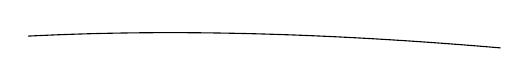
\begin{tikzpicture}\draw (0,0) .. controls (2,.1) and (4,.02) .. (6,-.15);\end{tikzpicture}}

\[
1+\operatorname{Sym}^{p^0}\qquad\xi_1,\tau_0\in\operatorname{Sym}^{p}
\]
$\xi$

\diagram{\begin{tikzcd}
A\otimes B\arrow[r]&C\qquad\mathbb F_p\text{-modules}
\end{tikzcd}}
\diagram{\begin{tikzcd}
K(A,i)\wedgeK(B,j)\arrow[r]&K(C,i+j)
\end{tikzcd}}
cup-products pairings

Le cup produit
\diagram{\begin{tikzcd}
K(\mathbb F_p,n)\wedgeK(\mathbb F_p,m)\arrow[r]&K(\mathbb F_p,m+n)
\end{tikzcd}}
induit en coh la comultiplication sur l'alg de Steenrod $A$ correspondant à la multiplication dans la duale
\diagram{\begin{tikzcd}
H^*(K(\mathbb F_p,n)\otimes H^*(K(\mathbb F_p,m)&H^*(K(\mathbb F_p,m+n),\mathbb F_p)\arrow[l]\\
A\otimes A&A\arrow[l]
\end{tikzcd}}
\mspage{368}

\scanpage{368}
\diagram{\begin{tikzcd}
A\arrow[r,"\varepsilon"]&\mathbb F_p
\end{tikzcd}}
\margin{$A$ $\mathbb F_p$ alg diff graduée aug sur $\mathbb F_p$}
\[
B(A)
\]
\[
\overline B(A):
\]
\diagram{\begin{tikzcd}[column sep=large]
A\otimes A\otimes A\arrow[r,shift left=3pt]\arrow[r]\arrow[r,shift right=3pt]&A\otimes A\arrow[r,shift left=2pt,"\mu"]\arrow[r,shift right=2pt,"1\otimes\varepsilon"']&A\arrow[l,bend right=55]\arrow[r]&ZEG
\end{tikzcd}}
\diagram{\begin{tikzcd}[column sep=large,execute at end picture={\draw (-3.4,.2) ellipse (5.5 and .65);}]
\underbrace{a\otimes\cdots\otimes a}_{n\text{ fois}}&A\otimes A\arrow[r,shift left=3pt]\arrow[r]\arrow[r,shift right=3pt]&A\arrow[r,shift left=2pt]\arrow[r,shift right=2pt]\arrow[d]&\mathbb F_p&\uline{ZBG}\\
&&a
\end{tikzcd}}
$A$ commutative

\diagram{\begin{tikzcd}[column sep=large,row sep=small]
{}\arrow[r,dash,shift left=4.5pt]\arrow[r,dash,shift left=1.5pt]\arrow[r,dash,shift right=1.5pt]\arrow[r,dash,shift right=4.5pt]&ZG^3\arrow[r,shift left=3pt]\arrow[r]\arrow[r,shift right=3pt]&ZG^2\arrow[r,shift left=2pt]\arrow[r,shift right=2pt]\arrow[d,dash]&|[circle,draw]|ZG\\
&&ZG\otimes ZG\arrow[ur,shift left=2pt]\arrow[ur,shift right=2pt]\\
&{}\arrow[ur,shift left=3pt]\arrow[ur]\arrow[ur,shift right=3pt]
\end{tikzcd}}
\margin{Bar Consts sur l'alg $ZG$}

\diagram{\begin{tikzcd}
A\otimes A&A\arrow[r,dash]&\mathbb Z
\end{tikzcd}}
\[
A=ZK(G,n)
\]
\[
\overline B(A)\sim ZBK(G,n)
\]
Structure d'algèbre de $\overline B(A)$

E Zilber

\margin{$A$ comm $\Rightarrow$\quad
\begin{tikzcd}
I\otimes A\otimes A\arrow[r]&A\quad\text{hom d'alg}
\end{tikzcd}}
\diagram{\begin{tikzcd}[column sep=large]
\overline B(A)\otimes\overline B(A)\arrow[r,shift left=2pt]&\overline B(A\otimes A)\arrow[l,shift left=2pt]\arrow[r]&\overline B(A)
\end{tikzcd}}
\mspage{369}

\scanpage{370}
Def de $K_2(R)$ de Milnor

\diagram{\begin{tikzcd}
E(R)\arrow[r,phantom,"\subset"]&GL(R)\arrow[r]&K_1(R)\arrow[r]&0
\end{tikzcd}}
\uline{Th}\quad $E(R)\equiv[E(R),E(R)]$

$R$ local\quad $E(R)=SL(R)$\quad (Whitehead)
\diagram{\begin{tikzcd}
E(R)\arrow[r,hook]&GL(R)\arrow[r,"\det"]&R^*\arrow[r]&0
\end{tikzcd}}
\margin{$1$}
\diagram{\begin{tikzcd}[column sep=small]
0\arrow[r]&K_2(R))\arrow[r]&\operatorname{St}(R)\arrow[r]\arrow[rr,bend left=18]&E(R)\arrow[r,hook]&Gl(R)\arrow[r]&K_1(R)\arrow[r]&0
\end{tikzcd}}
\[
\pi_1(E(R))=K_2(R)
\]
\[
BGl(R)^+
\]
\[
\operatorname{Ext}^2(\mathbb Z,G_m)
\]
Suite spectrale

\margin{$X$ un schéma}
\[
H^i_{\uuline{\mathrm{Zar}}}(X,\uuline{K}_j)\Rightarrow K_{j-i}(X)
\]
\[
H^i(X,\uuline{K}_{i})=\frac{i\text{-cycles}}{\text{equiv ratl}}.
\]
\diagram{\begin{tikzcd}[column sep=small]
0\arrow[r]&G_m\arrow[r]&i_*G_{mK}\arrow[r]&\displaystyle\bigoplus_{\text{pts de cod }1}\mathbb Z\arrow[r]&0
\end{tikzcd}}
\diagram{\begin{tikzcd}[column sep=small]
0\arrow[r]&\uuline{K}_1\arrow[r]&i_*\uuline{K}_1\arrow[r]&\displaystyle\bigoplus_{\text{pts }1}\uuline{K}_0\arrow[r]&0
\end{tikzcd}}
\diagram{\begin{tikzcd}[column sep=small]
0\arrow[r]&\uuline{K}_{i}\arrow[r]&i_*\uuline{K}_{i}\arrow[r]&\displaystyle\bigoplus_{\text{codim }1}j_*K_{i-1}\arrow[r]&\ldots\arrow[r]&\displaystyle\bigoplus_{\text{pts fermés}}s_*\mathbb Z\arrow[r]&0
\end{tikzcd}}
\[
\frac{H^0(X,s_*\mathbb Z)}{H^0(\qquad)}
\]
\mspage{371}

\scanpage{371}
\margin{\unsure{Thoh|Coh} \deleted{\unsure{K}} d'E-M}\mspage{I}

$H^*(K(\mathbb F_p\deleted{)},n),\mathbb F_p)={}$ Algebre anti com libre engendrée
\[
\left\{\begin{array}{ll}
\text{par Monomes admissible d'exces }<n & p=2\quad(\text{alg sym})\\
+\left\{\begin{array}{l}\text{''}\qquad\text{''}\qquad <n\\
\text{''}\qquad\text{''}\quad\text{d'exces }=n\ \text{qui se termine par }\beta
\end{array}\right. &p\ne2
\end{array}\right.
\]
\[
\begin{aligned}
i>0&\qquad\deg\xi_i=2p^i-2\\
j\geq0&\qquad\deg\tau_i=2p^i-1\\
\operatorname{Sym}(\xi_i)\otimes\Lambda(\xi_j)&\quad A_*\quad\text{\uline{l'algebre duale}}
\end{aligned}
\]
\[
A=\frac{\mathbb F_p[P^i,\beta]}{P^0=1,\ \text{Adem}}
\qquad \deg P^i=2i(p-1)\qquad\deg\beta\ \ 1
\]
\[
\begin{aligned}
&\operatorname{Sym}(\xi_i)\quad i>0\quad p=2&&A=\frac{\mathbb F_2[\operatorname{Sq}^i]}{\operatorname{Sq}^0=1,\ \text{Adem en car }2}\\
&\deg\xi_i=2^i-1,&&\deg\operatorname{Sq}^i=i\\
&&&\operatorname{Sq}^a\operatorname{Sq}^b
=\overset{a<2b}{\sum_{j=0}^{\prime\prime}}(\quad)\operatorname{Sq}^{a+b-j}\operatorname{Sq}^j
\end{aligned}
\]
\figure{\begin{tikzpicture}\draw (0,0).. controls (.55,1.6) and (.55,2.7)..(.7,4);\end{tikzpicture}}
\[
\begin{aligned}
\text{\textcircled{1}}\quad&H_{*}(K(\mathbb F_p,n),\mathbb F_p)\\
\text{\textcircled{2}}\quad&H_{*}(K(\mathbb Z,n),\mathbb F_p)\\
3\quad&H_{*}(K(\mathbb F_p,n),\mathbb Z)\\
4\quad&H_{*}(K(\mathbb Z,n),\mathbb Z)\qquad\swarrow
\end{aligned}
\qquad K(M\times N,n)\sim K(M,n)\times K(N,n)
\]
\margin{$G$\quad $\deleted{A}R$ \inserted{une $\mathbb F_p$-algebre} des \deleted{groupes} car $p$}
$H^*(K(G,n),\deleted{A}R)$ alg anticom libre sur le module \deleted{\unsure{libre}}
\[
\operatorname{Hom}(G,\deleted{A}R)\otimes_{\mathbb F_p}(\text{partie de } A\ \text{\uuline{d'exces}}<n)
\]
l'homologie est entierement de \uuline{torsion premiere}.

\unsure{Grau}
\[
H_*(K(G,n),\mathbb Z)=\bigoplus G/pG\oplus {}_pG
\]
$G$ abelien quelconque

Ex :
\[
\left.\begin{aligned}
H_{n+2}(K(G,n),\mathbb Z)&=G/2G\\
H_{n+3}(K(G,n),\mathbb Z)&={}_2G\\
n+4\qquad &=G/2G\oplus G/3G\\
n+5\qquad &={}_2G+{}_3G
\end{aligned}\right.
\]
\figure{\begin{tikzpicture}\draw (0,0).. controls (1.1,.9) and (1.2,1.8)..(1.3,2.7);\end{tikzpicture}}
dans la partie stable $H_{n+i}(K(G,n))$\quad $0\leq i<n$.

Bokstein
\[
\mathbb Z\xrightarrow{p}\mathbb Z\longrightarrow\mathbb Z/p
\]
\diagram{\begin{tikzcd}[column sep=tiny,row sep=small, font=\scriptsize]
{}\arrow[r,"0=p"]& H_*K(\mathbb F_p,n),\mathbb Z)\arrow[r]&
H_*(K(\mathbb F_p),\mathbb F_p)\arrow[r]\arrow[dr,"{\beta_{\deleted{*}1}}"']&
H_{*-1}(K(\mathbb F_p)\,\mathbb Z)\arrow[r,"p=0"]\arrow[d]\arrow[dr]&{}\\
0\arrow[ur]&&&H_{*-1}(K(\mathbb F_p),\mathbb F_p)&0
\end{tikzcd}}
Puisque mult par $p=0$, il suffit de \deleted{determiner} expliciter $\beta_*$ sur l'algebre $A_*$

\unsure{Deprême|De même} $K(\mathbb Z,n)\longrightarrow K(\mathbb Z,n)\longrightarrow K(\mathbb F_p,n)$ induit en deg $<2n$ une suite exacte (à partir de suite de Leray) :
\inserted{qui est courte pour la meme raison que ci-dessus.}
\diagram{\begin{tikzcd}[column sep=tiny,row sep=small, font=\scriptsize]
0\arrow[r]&H_*(K(\mathbb Z,n),\mathbb F_p)\arrow[r]&
H_{\deleted{\unsure{j}}*}(K(\mathbb F_p,n),\mathbb F_p)\arrow[r]\arrow[dr,"\beta_2"']&
H_{*-1}(K(\mathbb Z,n),\mathbb F_p)\arrow[r]\arrow[d]&0\\
&&&H_{*-1}(K(\mathbb F_p,n),\mathbb F_p)&
\end{tikzcd}}
les 2 $\beta_i$ \deleted{est une} \inserted{sont des} derivation sur l'algebre graduée $A_*$
\[
\operatorname{Sym}(\xi_i)\otimes\Lambda(\tau_i)\qquad\unsure{\zeta|\tau}
\]
\figure{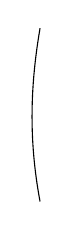
\begin{tikzpicture}\draw (0,0).. controls (-.15,.8) and (-.12,1.5)..(0,2.2);\end{tikzpicture}}
l'un des 2 $\beta_i$ :
\[
\begin{aligned}
&\tau_0\longrightarrow1\\
&\left\{\begin{aligned}\tau_i&\longrightarrow0\qquad i\ne0\\
\xi_j&\longrightarrow0\qquad j>0\end{aligned}\right.
\end{aligned}
\]
Conclusion \quad $H_*(K(\mathbb F_p,n),\mathbb Z)={}$ \deleted{l'autre} l'alg à puiss div libre eng par la partie d'exces $<n$ de
$\left\{\underset{\substack{i>0\\j>0}}{\operatorname{Sym}(\xi_i)\otimes\Lambda(\tau_j)}\right\}$

$H_*(K(\mathbb Z,n),\deleted{\mathbb F_p}\mathbb Z)$ : $\beta_2$ :
$\left\{\begin{aligned}\tau_j&\longrightarrow\xi_j\\ \xi_j&\longrightarrow0\end{aligned}\right\}$.

$\beta_2$ agit sur $H_*(K(\mathbb F_p,n),\mathbb Z)\xrightarrow{\beta_2}H_*(K(\mathbb F_p,n),\mathbb Z)$

C'est une derivation (anti com) :
\[
\begin{aligned}\tau_j&\longrightarrow\xi_j\\ \xi_j&\longrightarrow0\end{aligned}
\]
\[
\operatorname{Im}\beta_2=\ker\beta_2=H_*(K(\mathbb Z,n),\mathbb Z)_{(p)} .
\]
\figure{\begin{tikzpicture}\draw (0,0)--(1.2,0);\end{tikzpicture}}
La conjugaison $c:A\longrightarrow A$\quad $:A_*\longrightarrow A_*$ est explicitée dans Steenrod

Elle transforme l'un des $\beta$ dans l'autre et transporte la sous algebre (partie stable de) :
\diagram{\begin{tikzcd}[column sep=small,row sep=small]
(*)& H_*(K(\mathbb Z,n),\mathbb F_p)\arrow[r,"\sim"]\arrow[d,phantom,"\rotatebox{90}{$\subset$}"]&
H_*(K(\mathbb F_p,n),\mathbb Z)\arrow[dl,bend left=15]\\
&H_*(K(\mathbb F_p,n),\mathbb F_p)=A_*&
\end{tikzcd}}
\mspage{372}

\scanpage{372}\mspage{II}
\margin{Coh d'EM}
\deleted{\unsure{Th un|Th en} $\mathbb F_p$-modules}

Th (Cartan) : $G,H$ deux \deleted{anneaux} \inserted{groupes} (il fait des hyp sur $G$ et $H$),)
\[
H_*(K(G,n),H)\simeq H_*(K(H,n),G)\qquad\text{additif.}
\]
\uline{Dém} : Calcul.

\figure{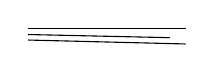
\begin{tikzpicture}\draw (0,0)--(2,0);\draw (0,-.08)--(1.8,-.12);\draw (0,-.15)--(2,-.2);\end{tikzpicture}}
$X$ un ensemble simplicial pointé.
\margin{$\pi_i(\mathbb ZX)=H_i(X)$}
\[
K(\mathbb Z,n)\wedge X\xrightarrow{A(X)}\deleted{\mathbb Z X}\mathbb Z^{+}(S^nX)
\]
\margin{$\mathbb Z^{+}(X,x)=\mathbb ZX/\mathbb Zx$}
$2n-1$ quasi isomorphisme.
\[
K(\mathbb Z,n)=\mathbb Z^{+}[S^n]
\]
\[
K(\mathbb Z,n)\wedge\underline X\longrightarrow K(\mathbb Z,n)\wedge\mathbb Z^+X
\]
\[
\left.\begin{aligned}
\mathbb Z\,X\times Y&\simeq\mathbb ZX\otimes\mathbb ZY\\
\mathbb Z^+(X\wedge Y)&\simeq\mathbb Z^+X\otimes\mathbb Z^+Y
\end{aligned}\right\}\quad
\begin{array}{l}EZ\\ EZ\ \text{pointé.}\end{array}
\]
\[
\mathbb Z^+(S^n)\wedge X\longrightarrow\mathbb Z^+(S^n)\wedge\mathbb Z^+X
\longrightarrow\mathbb Z^+(S^n)\otimes\mathbb Z^+X\xrightarrow{EZ}\mathbb Z^+(S^nX)
\]
\[
\pi_{n+r}(K(\mathbb Z,n)\wedge X)=\pi_{n+r}(\mathbb Z^+(S^nX))
=\widetilde H_{n+r}(S^nX)=\widetilde H_r(X)
\]
\uline{Dém} : $A(S^n)$
\[
\pi_i(K(\mathbb Z,n)\wedge S^m)\qquad
\mathbb Z^+(S^n\wedge S^m)=\mathbb Z^+(S^{n+m})
\]

\figure{\begin{tikzpicture}\node[inner sep=9pt] (box) {\begin{minipage}{.84\linewidth}
Ex de la dem 2 : interpretation du diagramme $(*)$ en bas de la page I
\diagram{\begin{tikzcd}[column sep=small,row sep=small]
K(\mathbb Z,n)\wedge K(\mathbb F_p,m)\arrow[r]\arrow[d,bend right=12]&
K(\mathbb F_p;m)\wedge K(\mathbb Z,n)\arrow[d]\\
K(\deleted{\mathbb Z}\mathbb F_p,n)\wedge K(\mathbb F_p,n)\arrow[r]&
K(\mathbb F_p,n)\wedge K(\mathbb F_p,n)
\end{tikzcd}}
\end{minipage}};\draw (box.north west) to[out=5,in=175] (box.north east) -- ([yshift=10pt]box.south east) to[out=-90,in=0] ([xshift=-24pt]box.south east) -- ([xshift=-24pt,yshift=-8pt]box.south east) to[out=200,in=0] ([yshift=-8pt]box.south west);\end{tikzpicture}}
\[
\begin{aligned}
S^m\wedge K(\mathbb Z,n)&\xrightarrow{\mathrm{qi}\ldots} K(\mathbb Z,n+m)\\
S^m&\longrightarrow\mathbb Z^+(S^m)=K(\mathbb Z,m)\\
S^m\wedge\deleted{K}K(\mathbb Z,n)&\longrightarrow K(\mathbb Z,m)\wedge K(\mathbb Z,n)\xrightarrow{\cup}K(\mathbb Z,n+m).
\end{aligned}
\]
Pt clef : $X\xrightarrow{h_r(\ )}\pi_{n+r}(K(\mathbb Z,n)\wedge X)$ est une th d'homologie partielle
\[
Y\hookrightarrow X\longrightarrow X/Y
\]
induit $h_r(Y)\longrightarrow h_r(X)\longrightarrow h_r(X/Y)\longrightarrow h_{r-1}(Y)\longrightarrow\ldots$

\uline{$r$ assez petit}.

Dem 2 du th de Cartan
\[
\pi_{i+m}(K(H,m)\wedge K(G,n)\simeq\pi_{i+n}(K(G,n)\wedge K(H,n))
\]
s'obtient par permutation des facteurs
\mspage{373}

\scanpage{373}
\uline{Resolutions canoniques d'un groupe abelien}

\[
X_*(G)\longrightarrow G\qquad X_i(G)=Z(G^n\times\mathbb Z^j)
\]
\diagram{\begin{tikzcd}[column sep=small]
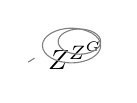
\begin{tikzpicture}[baseline=(z.base)]\node[inner sep=2pt] (z) {$\mathbb Z^{\mathbb Z^G}$};\draw[gray] (.05,.18) ellipse (.27 and .16);\draw[gray] (-.05,.13) ellipse (.37 and .22);\draw[gray] (-.6,-.08)--(-.52,-.03);\end{tikzpicture}\arrow[r,shift left=1ex]\arrow[r]\arrow[r,shift right=1ex] & 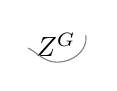
\begin{tikzpicture}[baseline=(z.base)]\node[inner sep=2pt] (z) {$\mathbb Z^G$};\draw[gray] (-.35,-.04) to[out=-30,in=180] (.02,-.22) to[out=0,in=-80] (.38,.12);\end{tikzpicture} & G
\end{tikzcd}}
\[
G\to G!\qquad H
\]
\margin{Pour tout $n$ on a une résolution simpliciale de $K(G,n)$ $\big\}$}
\diagram{\begin{tikzcd}
\mathbb Z^{\mathbb Z K(G,n)}\arrow[r,shift left=1ex]\arrow[r]\arrow[r,shift right=1ex]
&\mathbb Z^{K(G,n)}\arrow[l,shift left=2ex]\arrow[l,shift right=2ex]
\end{tikzcd}}
\[
K(G,n)=G\otimes_{\mathbb Z}\Lambda^n\Psi\qquad n\ \deleted{\text{large}}\ \text{grand}
\]
\[
\begin{aligned}
&r\text{-qis}\quad r<f(n,p)\quad K(\mathbb Z,n)\wedge K(G,p)\xrightarrow{\sim}\mathbb Z(S^n\wedge K(G,p))\longrightarrow\mathbb Z K(G,n+p)\\
&\hspace{7em} S^n\wedge K(G,p)\longrightarrow K(G,n+p).
\end{aligned}
\]
\[
\begin{aligned}
&K(\mathbb Z,p_1)\wedge K(\mathbb Z,p_2)\wedge\cdots\wedge K(\mathbb Z,p_r)\wedge K(G,p_{r+1})\ \sim\quad\mathbb Z^r K(G,\deleted{\unsure{n+}}p)\\
&\sum_{i=1}^{r+1}p_i=p
\end{aligned}
\]
\[
\begin{aligned}
&r\text{ qis}\qquad 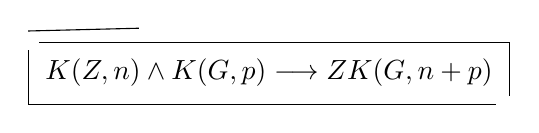
\begin{tikzpicture}[baseline=(b.base)]\node[inner sep=6pt] (b) {$K(\mathbb Z,n)\wedge K(G,p)\longrightarrow\mathbb Z K(G,n+p)$};\draw ([xshift=4pt]b.north west)--(b.north east)--([yshift=3pt]b.south east);\draw ([yshift=-3pt]b.north west)--(b.south west)--([xshift=-5pt]b.south east);\draw ([yshift=4pt]b.north west)--([xshift=40pt,yshift=5pt]b.north west);\end{tikzpicture}\\
&r=\min(n+2p-1,\,2n+p-1)
\end{aligned}
\]
\[
K(\mathbb Z,n)\wedge X\longrightarrow\mathbb Z[S^n\wedge X]
\]
\[
\deleted{K(\mathbb Z,p)\wedge}
\]
\diagram{\begin{tikzcd}[column sep=small]
K(\mathbb Z,n)\wedge K(\mathbb Z,m)\wedge K(\deleted{\mathbb Z}G,p)\arrow[r] & \mathbb Z[S^n\wedge K(\mathbb Z,n)\wedge K(G,p)]\arrow[d]\\
&\mathbb Z[K(\mathbb Z,n+m)\wedge K(G,p)]\arrow[d]\\
&\mathbb Z[\mathbb Z\deleted{\unsure{K}}[S^{n+m}\wedge K(G,p)]]\arrow[d]\\
&\mathbb Z[\mathbb Z K(G,n+m+p)]
\end{tikzcd}}
\mspage{374}

\scanpage{374}
\uuline{Foncteurs derives droits de Sym.}
\[
H^q(X,R)\simeq\underbrace{H^q(X,\mathbb F_p)}\otimes_{\mathbb F_p}R
\]
$\Theta\in\mathscr A=$ algebre de Steenrod
\[
\begin{aligned}
\underbrace{P_R^i}_{\substack{\text{construit}\\\text{par Steenrod}}}
 &=P^i\otimes1\qquad i>0\qquad 2i(p-1)\\
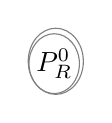
\begin{tikzpicture}[baseline=(z.base)]\node[inner sep=2pt] (z) {$P_R^0$};\draw[gray] (0,0) ellipse (.32 and .38);\draw[gray] (.02,.03) ellipse (.35 and .42);\end{tikzpicture}&\simeq\underbrace{P^0}_{1}\otimes F
\end{aligned}
\]
\[
G_a\otimes(\Lambda^n\Psi)\qquad G_a=\text{Fais structural de }(\mathrm{Sch}/\mathbb F_p)
\]
\figure{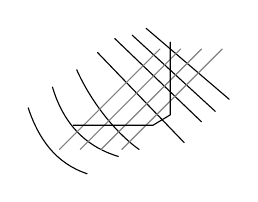
\begin{tikzpicture}[scale=.44,line cap=round]
\draw (0,.2)..controls (.3,-.7) and (.8,-1.4)..(1.7,-1.7);
\draw (.7,.8)..controls (1,-.2) and (1.6,-.9)..(2.6,-1.2);
\draw (1.4,1.3)..controls (1.8,.4) and (2.5,-.5)..(3.2,-1);
\draw (2,1.8)--(4.5,-.8); \draw (2.5,2.2)--(5,-.2);
\draw (3,2.3)--(5.4,.1); \draw (3.4,2.5)--(5.8,.45);
\foreach \x in {0,.6,1.2,1.8}{\draw[gray,thin] (\x+.9,-1)--(\x+3.8,1.9);}
\draw (1.3,-.3)--(3.6,-.3)--(4.1,0)--(4.1,2.1);
\end{tikzpicture}}
\figure{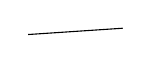
\begin{tikzpicture}\draw (0,0)--(1.2,.08);\end{tikzpicture}}
\[
\begin{aligned}
H^*(K(G_a,n),G_a)&=\text{Cl. les op}\\
\mathbb H^*(\mathbb Z[K(G_a,n)]^{\sim},G_a)&
\end{aligned}
\]
Illusie $X\text{ cat }D,(T)$ cat derivée des fais simpl\qquad $F$ objet abelien
\diagram{\begin{tikzcd}[column sep=small]
&\mathbb H^*(X,F^{*})=[X,K(F,n)]\\
H^j(X_i,F)\arrow[ur,Rightarrow]& X'\arrow[r]\arrow[d] & K(F,n)\\
&X
\end{tikzcd}}
\margin{Epstein L. Operations in homological algebra\par Invent. Math. 1 (1966)}

\figure{\begin{tikzpicture}\draw[->] (0,1.1) to[out=-100,in=170] (.3,0);\end{tikzpicture}}
Illusie p 69\qquad 3.2.1.19 -- 3.2.1.18
\[
\begin{aligned}
&\mathcal E xt^{p}(\Lambda(X),F)=\lim_{\substack{X'\to X\\\mathrm{qis}\\\text{fibrant}}}[X',K(F,p)]\\
&\text{def }''\, \mathbb H^p(X,F)
\end{aligned}
\]
\[
\mathcal E xt^p(\Lambda(-),F)\longrightarrow\operatorname{Ext}^q(\Lambda(\ ),G)
\]
Op coh de type $(F,p,G,q)$ sont class par $\mathbb H^q(K(F,p),G)$
\margin{$ZX\xrightarrow{f}K(A,q$}

\[
\mathbb H^n(K(G_a,m),G_a)=R^n\operatorname{Sym}(\mathbb F_p[m])
=\text{dual de }L^n\Gamma\,\deleted{\mathrm{Hom}}(\mathbb F_p[m])
\]
\uline{Theoreme} : Soit $\mathscr A$ l'algebre sur $\mathbb F_p$ eng par $P^i$\qquad
$\deg P^i=2i(p-1)$\qquad $i\geq0$ sat aux relations d'Adem (mais non à $P^0=1$).
\[
\mathbb H^*(K(\deleted{G_a}\mathcal O,m),\deleted{G_a}\mathcal O)
\]
est l'alg anticomm libre engendrée par les monomes admissibles de $\mathscr A$ d'exces $<n$.
\margin{\figure{\begin{tikzpicture}\draw (0,0)--(0,.65);\draw (0,-.1)--(.03,-.22);\end{tikzpicture}}$H^*(K(\mathbb F_{p^h},n),\mathbb F_{p^h})$}

\uline{Dém} : Comme dans le cas classique, il suffit de calculer 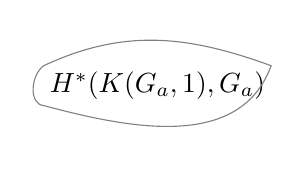
\begin{tikzpicture}[baseline=(h.base)]\node[inner sep=2pt] (h) {$H^*(K(G_a,1),G_a)$};\draw[gray] (h.north west) to[out=-145,in=175] (h.south west) to[out=-15,in=-110] (h.north east) to[out=160,in=25] (h.north west);\end{tikzpicture} et de grimper en utilisant le th de Borel et la suite sp de Leray associée à
\diagram{\begin{tikzcd}
K(G_a,n-1)\arrow[r]& *\arrow[d]\\
&K(G_a,n)
\end{tikzcd}}
\figure{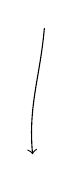
\begin{tikzpicture}\draw[->] (.15,1.6) to[out=-95,in=95] (0,0);\end{tikzpicture}} Lazard : Coh de l'analyseur classique dans ``Lois de groupes formels et analyseurs'' Ann ENS

\margin{$R$ anneau de car $p\geq0$\par $H^*(K(R,\unsure{m|n}),R)=$ Alg anticomm libre /$R$ eng par $\operatorname{Hom}_{\rm Ab}(R,R)$-module libre eng par les monomes admissibles $f\in\operatorname{Hom}(R,R)$}
\margin{$\oplus\ P^If\iota_n$\par $\underset{\rotatebox{90}{$\in$}\,x}{H^*(X,\mathcal O)}\longrightarrow\underset{P^Ix}{H^*(X,\mathcal O)}$\par $\mathrm{Hom}$}
\diagram{\begin{tikzcd}[row sep=small]
G_a^3&G_a\times G_a&G_a\\
&&\deleted{\operatorname{Sym}\mathbb F_p}\\
k[x,y,z]&k[x,y]\arrow[l]&k[x]\arrow[l]
\end{tikzcd}}
\[
\begin{aligned}
\iota_1&\in H^1(K(G_a,1),G_a)\\
\text{Witt}\ \longleftarrow\ \beta&\in H^2(K(G_a,1),G_a)\\
0\to G_a\to W_2&\to G_a\to0\\
0\to\mathbb Z/p\to\mathbb Z/p^2&\to\mathbb Z/p\to0
\end{aligned}
\]
On se ramène au calcul de
\diagram{\begin{tikzcd}
&H^*(K(\mathbb F_{p^h};1),\mathbb F_{p^h})\\
x\in H^{n}(K(\mathcal O,m),\mathcal O)\arrow[ur]& {}\\
K(\mathcal O,m)\arrow[r]&K(\mathcal O,n)\\
K(R,m)\arrow[r]&K(R,n)\qquad\forall R/\mathbb F_p
\end{tikzcd}}
\figure{\begin{tikzpicture}\draw (0,0)--(8,0);\end{tikzpicture}}

représenté par des polynomes de deg $<p^h$ en chaque var
\[
x\in H^*(K(\mathcal O,n),\mathcal O)_h\xrightarrow{\text{injective}}\mathbb H^*(K(\mathbb F_{p^h},n),\mathbb F_{p^h})
\]
\mspage{376}

\scanpage{375}
\uuline{Calcul des $\operatorname{Ext}^i(G_a,G_a)$}

\uline{Prop} : Le $k[F]$-module $\operatorname{Ext}^i(G_a,G_a)$ (pour l'action de $\operatorname{Hom}(G_a,G_a)$ à droite) est de $F$ torsion $(i>\deleted{0}1)$.

\uline{Cor} : (Milne) $G_a^\mathrm{parf}=$ restriction de $G_a$ au site parfait /$k$
\[
\begin{aligned}
G_a^\mathrm{parf}&=\lim_{\substack{\longleftrightarrow\\ F}}G_a\\
\operatorname{Ext}^i(G_a^\mathrm{parf},G_a^\mathrm{parf})&=0\qquad i>1.
\end{aligned}
\]
\figure{\begin{tikzpicture}\draw[->] (.25,3.4) to[out=-115,in=125] (.45,0);\end{tikzpicture}}\uline{Dém} : On considere la suite spectrale du coefficient universel
\[
\forall\ \text{fais simpl }X:\ E_2^{i,j}=\operatorname{Ext}^i_{\mathbb F_p}(\underline H_j(X),F)\Longrightarrow \mathbb H^{i+j}(X,F)
\]
En fait on va travailler dans la catégorie des fais de $\mathbb F_p$-modules

On travaille mod $F$ (au sens mod $\mathcal C$)
\[
\begin{aligned}
\operatorname{Hom}(G_a,G_a)&=k[F]\\
\operatorname{Ext}^1(G_a,G_a)&=0
\end{aligned}
\]
\margin{$\deleted{E^{*,j}}=\deleted{0}$\par $\deleted{j<n}$}

Dem par récurrence : On va considerer la s. spectrale précedente avec $X=K(G_a,n)$\qquad $\deleted{\operatorname{Ext}^i}$\quad $n$ grand.
\[
\begin{aligned}
E\qquad&\operatorname{Ext}^i(H_j(K(G_a,n)),G_a)\Longrightarrow \mathbb H^*(K(G_a,n),G_a)\\
E_2^{i,n}&=\operatorname{Ext}^i(H_n(K(G_a,n)\ G_a)\\
&\underset{\operatorname{Ext}^i(G_a,G_a)}{\shortparallel}
\end{aligned}
\]
\figure{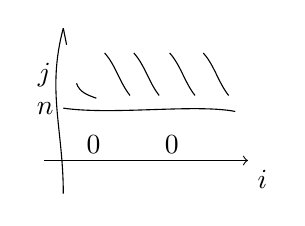
\begin{tikzpicture}[scale=.70]
\draw[->] (-.35,0)--(3.35,0) node[below right] {$i$};
\draw (0,-.6) to[out=90,in=-105] (0,2.4);\draw (0,2.4)--(.06,2.1);\node[left] at (-.05,1.55) {$j$};
\draw (0,.95) node[left] {$n$}..controls (.9,.82) and (2.4,1.03)..(3.12,.89);
\node at (.55,.29) {$0$};\node at (1.97,.29) {$0$};
\draw (.24,1.4) to[out=-70,in=160] (.60,1.13);\foreach \x in {.75,1.28,1.93,2.54}{\draw (\x,1.95)..controls (\x+.2,1.73) and (\x+.27,1.42)..(\x+.46,1.18);}
\end{tikzpicture}}
\[
\underline H_j(K(G_a,n)=\bigoplus G_a\qquad G_a\xrightarrow{p=0}G_a
\]
\mspage{377}

\scanpage{376}
\[
\operatorname{Ext}^i(H_j(K(G_a,n),G_a)\Longrightarrow\mathbb H^{i+j}(K(G_a,n),G_a)
\]
On raisonne par récurrence, mod $F$
\figure{\begin{tikzpicture}\draw (0,.16)--(.025,.05);\fill (.03,0) circle (.012);\end{tikzpicture}}
\diagram{\begin{tikzcd}[column sep=small]
\operatorname{Ext}^i(H_n(\deleted{K(G_a,n)},G_a)\arrow[r]
&H^{n+i}(K(G_a,n),G_a)\arrow[r]
&\operatorname{Hom}(H_{n+i}(K(G_a,n),G_a)\arrow[r]
&\operatorname{Ext}^{i+1}(G_a',G_a')\arrow[r,"\partial"]\arrow[d]
&H^{n+i+1}(K(G_a,n),G_a)\arrow[d,leftrightarrow]\\
0\arrow[ur]&{}&\underset{\bigoplus\operatorname{Hom}(G_a,G_a)}{\shortparallel}
&\underset{\underset{0}{\shortparallel}}{\operatorname{Ext}^{i+1}(\mathbb F_{p^h},\mathbb F_{p^h})}\arrow[r,"\partial"]
&H^{n+i+1}(K(\mathbb F_{p^h},n),\mathbb F_{p^h})
\end{tikzcd}}

\uline{Lemme 1} le edge homomorphism $\partial$ est nul.

\uline{lemme 2}\qquad $x$ un generateur de
\[
\begin{aligned}
H^{n+i}(K(G_a,n),G_a)&\longrightarrow\operatorname{Hom}(H_{n+i}(K(G_a,n),G_a)\\
P^I\iota_n&\hspace{4em}\shortparallel\\
\beta\underbrace{P^{i_1}\beta\cdots P^{i_r}}_{\text{longueur }r+s}\iota_n
 &\qquad\operatorname{Hom}(G_a\otimes H_{n+i}(K(\mathbb F_p,n)),G_a)\\
&\hspace{4em}\shortparallel\\
&\big(H^{n+i}(K(\mathbb F_p,n),\mathbb F_p)\otimes\operatorname{Hom}(G_a,G_a)\\
P^d\iota_n&\longrightarrow P^d\iota_n\otimes F
\end{aligned}
\]
Dém\qquad \unsure{on} le demontre pour $P^0\iota_n$

\figure{\begin{tikzpicture}\draw (0,0)--(1.0,0);\end{tikzpicture}}
\[
\begin{aligned}
\operatorname{Ext}_{\mathbb F_p}^*(G_a,G_a)\qquad
\operatorname{Ext}^{2i+1}(G_a,G_a)&=0\qquad \forall i\quad i>0\\
\operatorname{Ext}^{2i}(G_a,G_a)&=\frac{k[F]}{(F^d)}\qquad d=v_p(i).
\end{aligned}
\]
\diagram{\begin{tikzcd}[column sep=small,row sep=tiny]
\mathscr A\arrow[r]& A&\mathscr A\arrow[r]&\mathscr A\otimes\mathscr A\\
P^i\arrow[r]&P^i&P^i\arrow[r]&\displaystyle\sum_{j+k=i}P^j\otimes P^k\\
P^0\arrow[r]&1&{}&{}
\end{tikzcd}}
\figure{\begin{tikzpicture}\draw (0,0)--(1.5,0);\end{tikzpicture}}
\[
\operatorname{Ext}^i(\mathbb Z^{j}K(G_a,n),G_a)\Longrightarrow\operatorname{Ext}^{i+j}(G_a,G_a)
\]
\[
K(\mathbb Z)=K(\mathbb Z,m)\qquad n\ \text{grand}
\]
\diagram{\begin{tikzcd}[column sep=small]
Z^iK(G_a,n)\arrow[r,shift left=.6ex]\arrow[r,shift right=.6ex] & \cdots\arrow[r,shift left=1ex]\arrow[r]\arrow[r,shift right=1ex]
&ZZK(G_a,n)\arrow[r,shift left=.65ex]\arrow[r,shift right=.65ex]&ZK(G_a,n)
\end{tikzcd}}
\[
Z[Z^{j-1}K(G_a,n)]\sim Z[K(Z)\wedge K(Z)\wedge\cdots\wedge K(G_a,n)]
\]
\diagram{\begin{tikzcd}[column sep=small,row sep=small]
E_1\quad\ldots& A^{\otimes2}\otimes\mathscr A & A\otimes\mathscr A\arrow[l,shift left=1ex]\arrow[l]\arrow[l,shift right=1ex]&\mathscr A\arrow[l,shift left=.6ex]\arrow[l,shift right=.6ex]\\
\text{Dualement}\quad\ldots& A_*^{\otimes2}\otimes\mathscr A_*\arrow[r,shift left=1ex]\arrow[r]\arrow[r,shift right=1ex]& A_*\otimes\mathscr A_*\arrow[r,shift left=.6ex]\arrow[r,shift right=.6ex]&\mathscr A_*
\end{tikzcd}}
\[
\begin{aligned}
E_2^{i,j}&=\widetilde{\mathbb H}^{i}(K(Z)^{\wedge j-1}\wedge K(G_a),G_a)
\overset{\text{Kunneth}}{\sim}\widetilde{\mathbb H}^*(K(Z))^{\otimes j-1}\otimes\widetilde{\mathbb H}^*(K(G_a),G_a)\\
\mathbb H^*(K(\mathbb F_p),\mathbb F_p)&= A\\
\mathbb H^*(K(G_a),G_a)&=\mathscr A
\end{aligned}
\]
\[
E^2=\operatorname{Tor}^{A_*}(\mathscr A_*,\mathbb F_p)\Longrightarrow \unsure{E^2|t^2}\ \text{par Koszul}
\]
\mspage{378}

\cotefile{141}
\scanpage{2}
$V$ : \uline{W.d. noethérien}; Complet
\[
\operatorname{Spec}(V)\qquad k\ \text{corps \unsure{resid}}\qquad K\ \text{\unsure{corps fract\textsuperscript{s}|corps fractions}}
\]
Gpe galoisien $(K)$

a) $\operatorname{car}(\unsure{k|K})=0$\qquad \uuline{$k$ alg clos}.
\figure{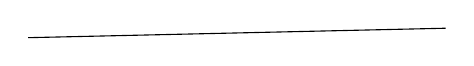
\begin{tikzpicture}\draw (0,0)--(5.3,.12);\end{tikzpicture}}
Les extens a $K$ sont \unsure{abel.} cyclique donc kummerienne.
\[
K^*/K^{*n}\simeq\mathbf Z/n\mathbf Z\qquad\text{(par la valuation)}
\]
Soit $\overline K$ clôture a $K$.
\diagram{\begin{tikzcd}[ampersand replacement=\&,column sep=small,row sep=small]
\Gamma(\overline K,K) \arrow[r,phantom,"\overset{\text{not}}{=}"] \& T_\infty(k) \arrow[r,phantom,"="] \& \displaystyle\varprojlim_n\underbrace{\mu_n(k)} \arrow[d,phantom,"\wr"] \& (\simeq\widehat{\mathbf Z})\\
\&\&\mathbf Z/n\mathbf Z
\end{tikzcd}}
\figure{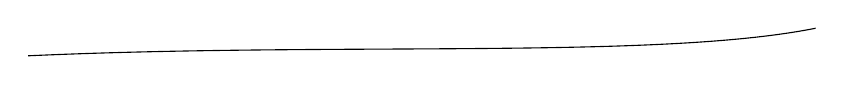
\begin{tikzpicture}\draw (0,0)..controls (4,.18) and (8,-.05)..(10,.35);\end{tikzpicture}}
si $k$ car $\unsure{\ne0}$ $V$ pas neces complet,
\[
\underset{\text{prem à }p}{\pi_1(K)}\longrightarrow\varprojlim_{n\text{ prem à }p}\mu_n(k)
\]
\mspage{1}

\scanpage{3}
UNIVERSITE

DES SCIENCES ET TECHNIQUES

DU LANGUEDOC

\texttt{------------}

Service de la Scolarité

MA/GJ

Diffusion : Liste A

N° : 5982

Montpellier, le 12 Novembre 1980

AVIS DE SOUTENANCE D'UNE THESE DE DOCTEUR INGENIEUR

CHIMIE ORGANIQUE PHYSIQUE

\texttt{-------------------------}

\uline{Nom et prénom du candidat} : MAUBERT Claude

\uline{Titre de la thèse} : ETUDES CINETIQUES DES TELOMERISATIONS AMORCEES PAR LES SELS DE METAUX DE TRANSITION ET LES GENERATEURS DE RADICAUX LIBRES.

\uline{Date, lieu et heure de soutenance prévus} : 18 NOVEMBRE 1980 à 10 Heures 30 mn

E.N.S.C.M.

\uline{Nom du Directeur de thèse} : Monsieur le Professeur Y. PIETRASANTA

\uline{Désignation du laboratoire où la thèse est préparée} : Laboratoire de Chimie Appliquée

E.N.S.C.M. 8 Rue de l'Ecole Normale, 34075 MONTPELLIER CEDEX.

\uline{Résumé de la thèse} :

Cette thèse est axée sur la détermination des paramètres permettant de contrôler les réactions de télomérisation. Le cas des télomérisations par catalyse rédox des acrylates de méthyle et d'éthyle avec le tétrachlorure de carbone a d'abord été étudié. Il est apparu que les chlorures ferriques et cuivriques étaient les réactifs prépondérants pour le contrôle des degrés de polymérisation. On a ensuite mis en évidence une diminution de l'importance du transfert lorsque la longueur de la chaîne augmentait. Le dernier volet de cette étude concerne la télomé-\\
risation de l'acétate de vinyle avec le tétrachloro 2,4,4,4, butanoate de méthyle amorcée par l'azobisisobutyronitile. La constante de transfert au télogène a été calculée ; on a également évalué le pourcentage des chaînes macromoléculaires comportant une molécule de télogène en extrémité.

\uline{Durée approximative des recherches ayant abouti à la thèse} : 3 ans

\uline{Composition du jury proposé} :
\begin{tabular}{ll}
MM.&REMPP P.\\
& BOUTEVIN B.\\
& DEISS W.J.\\
& GENESTE P.\\
& PIETRASANTA Y.
\end{tabular}

P. le Secrétaire Général,

L'Attachée d'Administration Universitaire,

\uline{P. Gentil}

\uline{A. GENTIL}
\mspage{2}

\scanpage{4}
\[
\bar s\in S\qquad
\pi_1(S,\bar s)\longrightarrow
\varprojlim_{n\ \text{``prem à }S\text{''}}\mu_n(S)
\]
$\bar s$ \uline{pt géométr.}

\figure{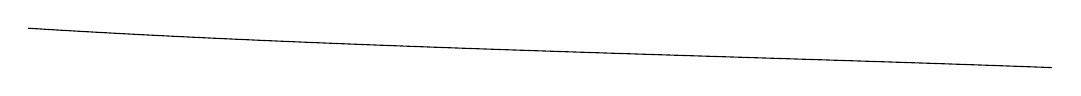
\begin{tikzpicture}
\draw (0,0.2) .. controls (4,-0.05) and (9,-0.15) .. (13,-0.3);
\end{tikzpicture}}

\diagram{\ensuremath{\begin{array}{ccccccccc}
1&\longrightarrow&\displaystyle\varprojlim_{n\ \text{prem à }p}\mu_n(\overline K)&\longmapsto&\pi_1(K)&\longrightarrow&\pi_1(\unsure{k|K})&\longrightarrow&1\\
&&&&&&\Vert&&\\
&&&&&&\pi_1(V)&&
\end{array}}}

\mspage{3}

\scanpage{5}
UNIVERSITE\\
DES SCIENCES ET TECHNIQUES\\
DU LANGUEDOC\\
\texttt{------------}\\
Service de la Scolarité\\
MA/GJ\\
Diffusion : Liste A\\
N\textdegree\ : 5890

Montpellier, le 7 Novembre 1980

AVIS DE SOUTENANCE D'UNE THESE DE DOCTORAT DE 3ème CYCLE

ECOLOGIE GENERALE ET APPLIQUEE Opt. ECOLOGIE TERRESTRE

\figure{\begin{tikzpicture}\draw (0,0)--(4,0);\end{tikzpicture}}

\uline{Nom et prénom du candidat} : MICHELLAND Dominique

\uline{Titre de la thèse} : SURVIE EN MILIEU INSULAIRE : QUELLE STRATEGIE ? LE CAS DES MESANGES EN CORSE.

\uline{Date, heure et lieu de soutenance prévus} :\\
17 NOVEMBRE 1980 à 15 Heures\\
Salle de cours n\textdegree\ 9 - USTL

\uline{Nom des Directeurs de thèse} :\\
MM. LEGENDRE et BLONDEL

\uline{Désignation du Laboratoire où la thèse est préparée} :\\
Laboratoire de Systématique et d'Ecologie Méditerranéennes

\uline{Résumé de la thèse} :

En Corse les populations de mésanges présentent un certain nombre de caractères démographiques et biométriques qui les différencient nettement des populations continentales.

A la lumière de la théorie de la biogéographie insulaire, cet ensemble d'observations peut s'interpréter comme le résultat de pressions de sélection de type K qui favorisent la survie des populations dans les milieux isolés et confinés.

Ce travail montre les répercussions, à l'échelle des populations, des importantes modifications, mises en évidence par ailleurs, de la structure et de la dynamique des communautés insulaires.

\uline{Durée approximative des recherches ayant abouti à la thèse} : 2 ans

\uline{Composition du jury proposé} :\\
MM. AMANIEU\\
\hspace*{2em}BLONDEL\\
\hspace*{2em}BOURLIERE\\
\hspace*{2em}THALER\\
\hspace*{2em}ISENMANN

P. le Secrétaire Général,\\
l' Attachée d'Administration Universitaire,

\uline{P. Gentil}\\
\uline{A. GENTIL}

\figure{
\begin{tikzpicture}
\draw (0.3,2.5) arc[start angle=100,end angle=245,radius=1.55];
\draw[gray] (-0.97,1.8) .. controls (-1.2,1.2) and (-0.8,0.3) .. (-0.6,0);
\node[rotate=62] at (-0.95,1.95) {\unsure{ACAD}};
\node[rotate=-41] at (0.05,1.05) {\unsure{SCIENCES}};
\end{tikzpicture}}

\mspage{4}

\scanpage{6}
\diagram{\begin{tikzcd}[ampersand replacement=\&,column sep=small]
0\arrow[r]\&H^0(S,\mu_n)\arrow[r,dash]\&H^0(S,G_m)\arrow[r,dash]\&H^1(S,\mu_n)\arrow[r]\&H^1(S,G_m)
\end{tikzcd}}

\diagram{\begin{tikzcd}[ampersand replacement=\&,column sep=large]
\mu_{1n}(S)\arrow[r]\&G_m(S)\arrow[r]\&G_m(S)\arrow[r]\&\operatorname{Rev}(S,\mu_n)\arrow[d]\\
\&\&\&\operatorname{Pic}(S)\arrow[d]\\
\&\&\&\unsure{\operatorname{Pic}}^{\otimes n}(S)
\end{tikzcd}}
% Second pass: the sign read \otimes n stands at the tip of the second vertical arrow, in the gap between
% "Pi" and "(S)" of the lowest term. Alternative reading (Hua batch-01, p. 5): \otimes n is the label of
% that arrow and its target is \operatorname{Pic}(S). The ink does not decide between the two.

\diagram{\begin{tikzcd}[ampersand replacement=\&,column sep=large]
0\arrow[r,dash]\&G_m(S)_n\arrow[r]\&\operatorname{Rev}(S,\mu_n)\arrow[r]\&\unsure{{}_n\operatorname{Pic}}(\unsure{A|S})\arrow[r]\&0
\end{tikzcd}}

\diagram{\begin{tikzcd}[ampersand replacement=\&,column sep=huge]
a\arrow[r,dash]\&\operatorname{Spec}\bigl(\underline{\mathcal O}_S[T]/T^n-a\bigr)
\end{tikzcd}}
\[
A[T]/(T^n-a)
\]

\mspage{5}

\scanpage{7}
UNIVERSITE\\
DES SCIENCES ET TECHNIQUES\\
DU LANGUEDOC\\
\texttt{------------}\\
Service de la Scolarité\\
MA/GJ\\
Diffusion : Liste A\\
N\textdegree\ : 5983

Montpellier, le 12 Novembre 1980

AVIS DE SOUTENANCE D'UNE THESE DE DOCTEUR INGENIEUR

SCIENCES ALIMENTAIRES Option GENIE ET TECHNOLOGIE ALIMENTAIRES -

FERMENTATIONS

\texttt{----------------------}

\uline{Nom et prénom du candidat} : COMTE Francis

\uline{Titre de la thèse} : Etude des isothermes d'adsorption de composés phénoliques.

\uline{Date, heure et lieu de soutenance prévus} : 18 NOVEMBRE 1980 à 15 Heures 30 mn\\
Salle de cours n\textdegree\ 9 - U.S.T.L.

\uline{Nom du Directeur de thèse} : Monsieur le Professeur J. CROUZET

\uline{Désignation du laboratoire où la thèse est préparée} : Biochimie Appliquée

\uline{Résumé de la thèse} :

Le tracé d'isothermes d'adsorption sur silice de composés phénoliques (acides benzoïque et salycilique) étudiés en qualité de modèles d'anthocyanes a été obtenu par des méthodes dynamiques mettant en oeuvre la chromatographie liquide haute performance.

Parmi les différentes méthodes utilisées par élution (profil de pic, maximum de pics) ou par analyse frontale (équilibre, profil de désorption) la technique du profil de désorption est la plus rapide mais sujette à cautions. La méthode la plus fiable, quoique la plus longue, est la méthode à l'équilibre, c'est d'ailleurs la seule méthode qui autorise le tracé des isothermes individuelles par adsorption d'un mélange.

Par modélisation nous avons pu montrer que le meilleur accord était obtenu avec le modèle de SCOTT et KUCERA qui décrivent une adsorption en double couche.
En dépit des difficultés qui se sont liées à l'intervention de phénomènes propres à la chromatographie liquide et qui contribuent à la déformation des pics il nous a été possible de montrer que la capacité d'adsorption de la silice était supérieure pour l'acide ben-\\
zoïque. Ceci est confirmé par l'étude de l'adsorption mixte sans que l'on puisse parler d'adsorption spécifique ou de sélectivité de l'absorbant.

\uline{Durée approximative des recherches ayant abouti à la thèse} : 3 ans

\uline{Composition du jury proposé} :\\
MM. ROUZAUD J.\\
\hspace*{2em}CROUZET J.\\
\hspace*{2em}GOMA G.\\
\hspace*{2em}COMBE P.

P. le Secrétaire Général,\\
L'Attachée d'Administration Universitaire,

\uline{P. Gentil}\\
\uline{A. GENTIL}

\figure{\begin{tikzpicture}
\draw[gray,densely dotted] (0.1,0.7)..controls(-0.3,0.3)and(-0.2,-0.1)..(0.05,-0.35);
\draw[gray] (0.13,0.65)--(0.17,0.25);
\draw[gray,densely dotted] (0.8,0.5)--(0.9,0.3);
\end{tikzpicture}}

\mspage{6}

\scanpage{8}
\uline{Thm 1} Soit $\pi$ groupe discret, $E$ revêtement $\pi$-principal d'un espace $B$.
Considérons pour \inserted{tout} espace $X$ l'application
\[
\operatorname{hot}(X,B)\xrightarrow{h_X}H^1(X,\pi)
\quad\bigl(\overset{\mathrm{df}}=\text{classes d'isom. de $\pi$-rev. princi-paux de $X$}\bigr)
\]
\figure{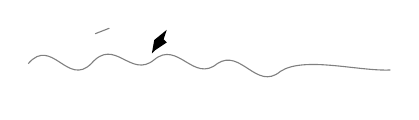
\begin{tikzpicture}
\draw[gray] (.85,.38)--(1.03,.45);
\fill (1.57,.13)--(1.6,.3)--(1.76,.43)--(1.72,.31)--(1.76,.27)--(1.61,.17)--cycle;
\draw[gray] (0,0) .. controls (.3,.35) and (.5,-.3) .. (.8,0)
.. controls (1.1,.35) and (1.3,-.2) .. (1.6,.05)
.. controls (1.9,.3) and (2.1,-.25) .. (2.4,0)
.. controls (2.7,.2) and (2.9,-.35) .. (3.2,-.1)
.. controls (3.5,.1) and (4.2,-.1) .. (4.6,-.08);
\end{tikzpicture}}
fonctorielle en $X$.
\figure{
\begin{tikzpicture}\draw (0,.1) .. controls (.12,-.08) and (.53,-.1) .. (.38,.1) -- (.12,.25) .. controls (.35,.13) and (.63,.03) .. (.48,.36) -- (.4,.55) .. controls (.43,.64) and (.7,.64) .. (.78,.78);\end{tikzpicture}}

Conditions équivalentes

1) $h$ est un isomorphisme de foncteurs,

\hspace*{2em}i.e. \deleted{\unsure{in}}\inserted{bi}jectif pour $\forall\ X$

(On dit alors que $(E,B,\pi)$ est un $\pi$-rev. universel, $B$ s'appelle ``l'espace classifiant'' pour $\pi$)

2) $E$ est contractile

\mspage{7}

\scanpage{9}
\uline{Thm 2} Pour $\forall\ \pi$ discret, il existe un $\pi$ fibré universel,
i.e. un espace classifiant (défini à isom unique près dans la cat. homotopique \begin{tikzpicture}[x=.25cm,y=.25cm,baseline=-.4ex]\fill (0,0) circle (.08);\draw (.3,-.02)..controls (.55,.06) and (.62,.04)..(.7,-.02)..controls (.8,-.11) and (.95,-.11)..(1.05,-.1);\end{tikzpicture})

Soit $X$ un espace sur lequel $\pi$ opère à \unsure{g.}
et prenons

\diagram{\begin{tikzcd}[ampersand replacement=\&,column sep=large]
\&E_\pi\times_\pi X\overset{\deleted{\unsure{E|df}}}{=}\underbrace{(E_\pi\times X)/\pi}\arrow[dl]\arrow[dr]\&\supsetX\\
B_\pi=E_\pi/\pi\&\&X/\underset{\deleted{E_\pi}}{\pi}
\end{tikzcd}}

\margin{\begin{tikzpicture}[scale=.45]\draw[gray] (0,0)--(.8,.35)--(.6,.65) (.8,.35)--(.4,.35) (.4,-.1)--(.42,-.4);\end{tikzpicture}}
\diagram{\begin{tikzcd}[ampersand replacement=\&,column sep=small]
\pi_2(B_\pi)\arrow[r]\arrow[d,equal]\&\pi_1(X)\arrow[r,dash]\&\pi_1(X,\pi)\arrow[r]\&\pi\arrow[r]\&\pi_0(\unsure{V|X})\arrow[d,equal]\\
0\&\&\&\&1
\end{tikzcd}}

\mspage{8}

\scanpage{10}
\[
\tilde x\in(\tilde X\supset\tilde K\supset\tilde S)\simeq C_{pq}
\qquad \uline{\Gamma_{pq}}\supset\Pi
\qquad\operatorname{Norm}(\Pi)/\Pi
\]
\figure{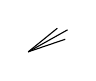
\begin{tikzpicture}\draw (0,0)--(.5,.28);\draw (0,0)--(.47,.16);\draw (0,0)--(.37,.30);\end{tikzpicture}}
\[
x\in\uline{X\supset K\supset S}\qquad\uline{p},\uline{q}
\]

\diagram{\begin{tikzcd}[ampersand replacement=\&,column sep=large]
\&\Gamma_{\infty\infty}\supset\Pi\arrow[dl]\arrow[d]\\
\Gamma_{\infty,3}\&\Gamma_{p,q}\supset\Pi
\end{tikzcd}}

\figure{\begin{tikzpicture}[x=.8cm,y=.8cm]
\draw (0,6)--(5.1,6)..controls(5.1,5.4)and(5.05,5)..(5.2,4.65);
\draw (5.05,4.5)--(11.5,4.5);
\draw (9.05,4.5)..controls(9.4,5.6)and(9.6,7.3)..(10.1,7.3);
\draw[line width=1.4pt] (9.05,4.5)--(9.4,4.35);
\node at (10.7,6.8) {$V\ni e$};
\node at (10.6,5.95) {$\uuline{\omega_1},\uuline{\omega_2}$};
\node at (10.65,5.15) {$\mathrm I(\omega_2/\omega_1)>0$};
\node at (2.3,5.65) {$C_{\infty,3}$};
\draw[->,thick] (2.3,5.25)--(2.3,2.6);
\draw (2.5,2.55)..controls(3.7,2.5)and(3.7,1.1)..(3.2,.7);
\draw (2.3,2.55)..controls(.7,2.1)and(1.1,.4)..(2.6,.45);
\draw (1.4,1.3)..controls(2,.95)and(2.9,.9)..(3.4,1.3);
\draw[dashed] (1.4,1.3)..controls(1.65,1.9)and(3,1.85)..(3.4,1.3);
\fill (2.28,1.05) circle(.018);\fill (3.13,1.1) circle(.014);
\fill (1.85,1.14) circle(.065);\fill (3,1.13) circle(.065);\fill (2.55,1.69) circle(.065);
\node at (7,3.95) {$\Gamma_{21}$};
\draw (8.9,3.45)..controls(8,3.55)and(7.7,2.7)..(7.8,2.4);
\draw (8.9,3.45)..controls(9.8,3.7)and(10.1,3.3)..(10,2.8);
\draw (7.8,2.7)..controls(8,1.7)and(8.8,1.7)..(9.8,2.6);
\draw (7.8,2.7)..controls(8.7,3.2)and(9.7,3.1)..(9.8,2.6);
\draw (7.8,2.4)..controls(7.75,1.3)and(8.2,1.1)..(8.65,.95);
\draw (10,3)..controls(10.05,1.4)and(9.7,1.05)..(9.1,.9);
\draw (7.8,2.7)--(9.3,3.67);
\draw (7.8,2.7)--(9.75,3.35)--(7.75,1.9)--(9.85,2.65)--(8.45,1.4)..controls(8.2,1.1)and(9.4,1.6)..(9.85,1.6);
\fill (8.95,3.45) circle(.065);\fill (9.1,1.98) circle(.065);\fill (9.05,.95) circle(.065);
\node at (11.1,3.65) {$\omega_1,\omega_2$};
\node at (11.2,2.85) {$\omega_2/\omega_1=\tau$};
\draw[line width=1.1pt] (5.8,4.4)--(5.83,4.28)--(5.77,4.3);
\node at (5.8,4.05) {$1$};
\node[anchor=north] at (5.8,3.55) {\diagram{\begin{tikzcd}[ampersand replacement=\&,row sep=small]
\Pi_1\arrow[d]\\
\Gamma^{\circ}_{\infty,3}=\operatorname{Sl}(7,\mathbf Z)/(\pm1)\arrow[d]\\
\mathfrak S_3\arrow[d]\\1
\end{tikzcd}}};
\end{tikzpicture}}

\diagram{\begin{tikzcd}[ampersand replacement=\&,row sep=small]
\{\sigma_0,\sigma_1,\sigma_2\mid\overline{\rho_{\delta}^{3}=1}\arrow[d,equal]\\
\Gamma_{\infty3}\supset\Pi\arrow[d,rightsquigarrow]\\
\rho_{\delta}\qquad\uline{\rho_{\delta}^p}
\end{tikzcd}}

\figure{\begin{tikzpicture}
\draw[gray] (.5,2.7)--(1.4,2.7);\fill (.5,2.7) circle(.02);\fill (1.4,2.7) circle(.02);
\fill (1.04,.54)--(1.36,.62)--(1.04,.7)--cycle;
\fill (1.78,2.41)--(2.06,2.22)--(1.91,2.48)--cycle;
\draw (1.1,0.6)..controls(-.4,.6)and(-.5,2.1)..(.8,2.4)..controls(2.8,2.9)and(2.6,.6)..(1.1,.6);
\draw[dashed] (-.1,1.8)--(-.1,.85);
\node at (.35,1.7) {$\times$};\node at (.4,1.38) {$0$};
\node at (.9,1.7) {$\times$};\node at (1.15,1.33) {$2^3.34$};
\fill (2,1.65) circle(.045);
\node at (2.8,1.5) {$C_{11}$};
\node at (1,.25) {$\unsure{R\ \text{quot}(p,q)|R_{(p,p',q,q')}}$};
\draw[->] (.1,0)--(.1,-.6);
\node[anchor=north] at (.1,-.7) {\diagram{\begin{tikzcd}[ampersand replacement=\&,row sep=large]
\Gamma_{p,q}\arrow[d]\\\Gamma_{p',q'}
\end{tikzcd}}};
\end{tikzpicture}}

\diagram{\begin{tikzcd}[ampersand replacement=\&,row sep=large]
C_{\infty3}\arrow[d]\\C_{p3}
\end{tikzcd}}

\diagram{\begin{tikzcd}[ampersand replacement=\&,row sep=large]
C_{pq}\arrow[d]\\C_{p',q'}\arrow[d,equal]\\C_{pq}/R
\end{tikzcd}}
\[
\begin{gathered}p'\mid p\\q'\mid q.\end{gathered}
\qquad
\begin{array}{cc}C_{21}&C_{12}\\&C_{11}\end{array}
\]

\mspage{9}

\scanpage{11}
Carte trouée
\diagram{\begin{tikzcd}[ampersand replacement=\&,column sep=small]
(X\arrow[d]\supset K\arrow[dr])\&\&\text{tels que}\\
\text{surf. top.}\&\begin{gathered}\text{sous-variété fermée}\\\text{de dim 1}\end{gathered}\&
\end{tikzcd}}

Tte comp. de $\operatorname{Déc}(X,K)$ est homéomorphe : un $D_n^*$

(disque troué standart, $1\leq n\leq+\infty$)

$\Pi_n$ pol. comb. ép. d'ordre $n$
\[
\uline{|\Pi_n|\times]0,1]}\supset|\Pi_n|\supset S_n
\qquad
\begin{gathered}\Pi_n:(S_n,A_n,R_n)\\S_n\subset|\Pi_n|\end{gathered}
\]
\[
D_n^*=|\Pi_n|\times]0,1]\setminus S_n
\]

\figure{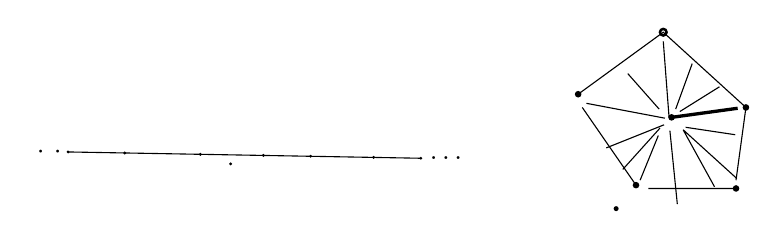
\begin{tikzpicture}[x=.8cm,y=.8cm]
\begin{scope}[shift={(7.9,3.15)},x=.0105cm,y=-.0105cm]
\draw (15,94)--(118,19)--(218,110)--(206,198) (204,208)--(100,208) (85,204)--(20,110);
\draw (125,122)--(118,30) (113,112)--(75,69) (120,123)--(25,105);
\draw (133,112)--(153,57) (138,115)--(186,85);
\draw[line width=1.2pt] (128,122)--(208,111);
\draw (145,134)--(205,143) (142,137)--(207,196) (142,137)--(180,206);
\draw (126,138)--(135,227) (112,144)--(90,198) (114,135)--(69,185) (119,131)--(49,159);
\draw[line width=.9pt] (118,19) circle(4);
\foreach \x/\y in {15/94,218/110,206/208,85/204,128/122}{\fill (\x,\y) circle(4);}
\end{scope}
\node at (-.3,1) {$\cdot\ \cdot$};
\draw (0,1)--(5.6,.9);
\foreach \x in {0,.9,2.1,3.1,3.85,4.85,5.6}{\fill (\x,{1-.1*\x/5.6}) circle(.025);}
\fill (2.58,.81) circle(.025);
\node at (6,.9) {$\ldots$};
\fill (8.7,.1) circle(.04);
\end{tikzpicture}}

\figure{\begin{tikzpicture}[x=.8cm,y=.8cm]
\draw[->] (3.4,6.2)--(1.3,5.55);
\draw[->] (2.55,5.75)--(2.2,6.35);
\draw (3.8,6.2)..controls(4.5,5.95)and(5.3,6)..(5.9,5.65);
\draw[->] (5.15,5.91)--(5.55,5.8);
\draw[->] (4.55,5.85)--(4.7,6.3);
\draw (6.08,5.48)--(6.34,5.1);
\draw[->,thick] (6.2,5.35)--(7.15,4.05);
\draw (7.1,4.25)..controls(7.4,3.9)and(7.5,3.6)..(7.45,3.5);
\draw (3.4,5.9)--(1.7,3);
\draw (5.15,4.9)--(5,4.4);\draw (4.9,4.2)--(3.65,2.1);
\draw (7.1,3.4)..controls(7,2.8)and(6.8,2.3)..(6.5,1.9);
\draw (7.6,3.3)..controls(7.85,2.3)and(7.5,1.8)..(7.65,1.2);
\node at (3.5,.8) {$E$};
\node at (1,.65) {$\uline{\sigma_0\ \sigma_1}\ \sigma_2$};
\draw (9.6,5.45) ellipse (1.02 and .94);
\draw (10.65,6.9)--(10.65,3.1);
\draw[thick] (9.6,5.45)--(10.65,5.4);
\draw (8.8,4.85)--(10.75,6.25);
\draw (8.8,4.85)--(8.91,5.03)--(8.96,4.86)--(9.03,5.14)--(9.09,4.98)--(9.16,5.22)--(9.22,5.07)--(9.29,5.31)--(9.35,5.18)--(9.48,5.4);
\foreach \x/\y in {9.45/6.38,8.65/5.75,8.8/4.85,9.82/4.51,10.63/5.16,10.65/5.4,10.42/6.0,9.6/5.45}{\fill (\x,\y) circle(.045);}
\fill (9.15,4.26) circle(.018);\fill (9.05,4.06) circle(.02);
\draw[->,thick] (9.4,4.53)--(9,4.62);
\node at (11.65,5.7) {$\pm\frac1n$};
\draw (9.45,1.95) ellipse (1.15 and 1.1);
\draw[line width=2pt] (9.25,3.04) arc[start angle=100,end angle=38,x radius=1.15,y radius=1.1];
\draw[line width=2pt] (10.52,1.58)--(10.35,1.19);
\draw[line width=2pt] (10.05,1.02)..controls(9.9,.8)and(9.65,.81)..(9.4,.82);
\draw[line width=2pt] (8.31,2.25)--(8.31,1.55);
\draw[->,thick] (8.32,2.57)--(8.65,2.8);
\draw (8.3,2.52)--(8.45,2.32);\draw[thick] (8.19,2.2)--(8.43,2.22);
\draw[->] (9.4,1.4)..controls(10,1.6)and(10,1.9)..(9.9,2.2);
\draw[dashed] (12.65,1.48) circle(.25);
\draw[gray] (12.9,.95)..controls(13.1,1.01)and(13.17,.88)..(13.17,.8) (12.66,.76)--(12.7,.84);
\foreach \x/\y in {12.9/.96,13.17/.8,12.66/.57,13.02/.35}{\fill (\x,\y) circle(.02);}
\draw (13.1,-.15) circle(.17);\draw[gray] (13.12,-.13) circle(.17);
\end{tikzpicture}}

\figure{\begin{tikzpicture}
\draw (3.6,4)--(6.6,4)--(6.55,2.95) (3.45,3.8)--(3.5,2.98)..controls(4.3,2.72)and(5.6,2.85)..(6.3,2.85);
\node[inner sep=8pt] at (5,3.5) {$\operatorname{Déc}(\hat X,\omega)$};
\node at (8.4,3.4) {$\tilde X-F$};
\draw (2.1,3.55)--(2.4,3.2)--(3.8,2.55)--(3.5,.9)--(3.3,.95) (3.18,.98)--(2,{.2+1})--(1.65,2.65);
\draw (2.1,3.55)--(1.85,4.1);\draw (2.1,3.55)--(2.4,3.95);
\draw (1.65,2.65)--(.6,2.75);\draw (1.65,2.65)--(1.55,3.3)--(2.1,3.55);
\draw (2.4,3.2)--(1.65,2.65);\fill (1.55,3.3) circle(.025);\fill (2.1,3.55) circle(.025);
\draw (3.8,2.55)--(4.5,3);\draw (3.5,.9)--(3.8,.5);\draw (2,1.2)--(1.7,.5);
\foreach \x/\y in {2.4/3.2,3.8/2.55,3.5/.9,2/1.2,1.65/2.65}{\fill (\x,\y) circle(.04);\draw (\x,\y) circle(.19);}
\draw (2.7,2.1) circle(.15);\fill (2.7,2.1) circle(.035);
\draw (5.3,2)--(5.8,2.45);\draw (5.3,2)--(5.25,2.45);\draw (5.3,2)--(4.95,2.2);\draw (5.3,2)--(4.9,1.65);\draw (5.3,2)--(5.4,1.65);\draw (5.3,2)--(5.85,1.95);
\end{tikzpicture}}

\mspage{10}

\scanpage{12}
\[
n\left\{\begin{array}{ll}L&d\text{ gén.}\\\cup&\\L'&d'\text{ gén}\end{array}\right.
\qquad\begin{gathered}(d'-1)=n(d-1)\\2=2.1\end{gathered}
\qquad\textcircled{1}
\]

\figure{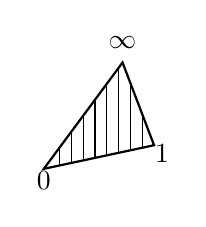
\begin{tikzpicture}
\draw[thick] (0,0)--(1,1.35)--(1.4,.3)--cycle;
\foreach \x in {.2,.35,.5,.65,.8,.95,1.1,1.25}{\draw (\x,{.214*\x})--(\x,{min(1.35*\x,3.975-2.625*\x)});}
\node at (0,-.15) {$0$};\node at (1.5,.2) {$1$};\node at (1,1.6) {$\infty$};
\end{tikzpicture}}

\figure{\begin{tikzpicture}
\draw (0,0)..controls(.4,1.1)and(1.7,.8)..(0,0);
\draw (0,0)..controls(1.2,.25)and(1.8,-.4)..(0,0);
\draw (0,0)..controls(-.4,-.8)and(.8,-1.1)..(0,0);
\fill (0,0) circle(.04);
\end{tikzpicture}}

\[
\begin{array}{lll}L\simeq\pi_1(X)&&1-d\\\cup&&\\L'\simeq\pi_1(X')&&1-d'\end{array}
\]
\[
\pi^+
\]
\diagram{\begin{tikzcd}[ampersand replacement=\&,column sep=small,row sep=small]
\rho_0\arrow[d,maps to]\&\rho_1\arrow[dd,maps to]\&\rho_\infty\arrow[d,maps to,harpoon]\\
\rho_0^{-1}.\&\&\rho_\infty^{-1}\\
\&\rho_\infty\rho_0\&
\end{tikzcd}}

\[
\pi
\]
\diagram{\begin{tikzcd}[ampersand replacement=\&,column sep=large,row sep=large]
\&\&\margin{\text{avec }\varinjlim}\\
\operatorname{Ens}(\unsure{\pi|E})\arrow[r,"\begin{gathered}F\\\text{commutant}\end{gathered}","\text{aux }\varinjlim"']\arrow[d,leftrightarrow]\&C\arrow[r,bend right=12,"G\text{ commute}","\text{aux }\varinjlim"']\arrow[ur,bend left=15,dash]\&C'\\
\phantom{X}\&X\quad\pi\text{-objet }\inserted{\text{\unsure{à|:} droite}}\text{ de }C\&
\end{tikzcd}}
\margin{$(\simeq\operatorname{Ens}(\pi'))$}

\[
F\longmapsto F(\underline{\pi_s})
\]
\[
X\longmapsto F_X:E\longmapsto\underbrace{X\times_\pi}_{\in\operatorname{Ob}C}E
\]
\[
\operatorname{Hom}_C\bigl(X\times_\pi E,
\underset{\substack{\rotatebox{-90}{\ensuremath{\in}}\\\operatorname{Ob}C}}{\deleted{E}\inserted{Y}}\bigr)
\simeq\operatorname{Hom}_\pi\bigl(E,\operatorname{Hom}(X,Y)\bigr)
\]
\[
E\simeq\coprod_{i\in I}\pi/H_i
\]
\[
X\times_\pi E=\coprod_i\underbrace{X\times_\pi(\pi_s/H_i)}_{X/H_i}
\]

\mspage{11}

\scanpage{13}
\uline{Ex} $C=\operatorname{Ens}(\pi')$
\margin{\textcircled{2}}

\diagram{\begin{tikzcd}[ampersand replacement=\&,row sep=large]
\underset{\substack{\tikz[baseline=-.3ex]\draw (0,.17)..controls(-.08,.03)and(-.05,-.06)..(.03,-.09);\text{commutant}\\\text{aux }\varinjlim}}{\underline{\operatorname{Hom}}_!}\bigl(\operatorname{Ens}(\pi),\operatorname{Ens}(\pi')\bigr)\arrow[r,phantom,"\simeq"]\&{}_{\pi'}\operatorname{Ens}_\pi\arrow[d,phantom,"\rotatebox{90}{$\in$}"]\\
\&{}_{\pi'}X_\pi
\end{tikzcd}}


\diagram{\begin{tikzcd}[ampersand replacement=\&,column sep=large]
X\arrow[d,leftrightarrow]\&\operatorname{Ens}(\pi)\arrow[d,phantom,"\rotatebox{90}{$\in$}"]\\
F:\&E\arrow[r,maps to]\&X\times_\pi E
\end{tikzcd}}

\uline{Proposition} Pour que $F$ soit exact à gauche,
il f. et s. que $X$ soit un $\pi$-torseur à droite.
\figure{\begin{tikzpicture}\draw (0,0)--(.05,-2.1);\end{tikzpicture}}

$X$ torseur sous $\pi$
\[
{}^X\pi\overset{\mathrm{df}}=X\times_\pi\operatorname{int}(\pi)=\operatorname{Aut}_\pi(X)
\]
\[
\pi'\longrightarrow\operatorname{Aut}_\pi(X)
\]

\uline{Corollaire} Pour que $F$ soit équivalence, il f et s que
$\pi'\xrightarrow{\sim}\operatorname{Aut}_\pi(X)$, i.e. que $X$ soit un
bitorseur sous $\pi',\pi$; donc

\diagram{\begin{tikzcd}[ampersand replacement=\&,column sep=large,row sep=large]
\underline{\operatorname{Équiv}}\bigl(\operatorname{Ens}(\pi),\operatorname{Ens}(\pi')\bigr)\arrow[r,phantom,"\approxeq"]\arrow[d,"\wr"',"u\longmapsto u^{[-1]}"]\&\operatorname{BiL}(\pi',\pi^{\unsure{3|*}})\arrow[d,"u"]\\
\underline{\operatorname{Equiv}}\bigl(\operatorname{Ens}(\pi'),\operatorname{Ens}(\pi)\bigr)\arrow[r,"\approx"]\&\operatorname{Bit}(\pi,\pi')
\end{tikzcd}}

\mspage{12}

\scanpage{14}
\deleted{\uline{\unsure{Bitinvol}}}
\[
{}_\pi X_\pi\qquad X\circ X\overset{\mu}{\xleftarrow{\sim}}1
\]
\[
\lambda e=e\lambda\qquad\forall\lambda\in\pi
\]
\[
\underline{\operatorname{Bitinvol}}(\pi)\xrightarrow{\approx}
\underline{\operatorname{Invol}}\bigl(\operatorname{Ens}(\pi)\bigr)
\]
\[
\xrightarrow{\approx}\underline{\operatorname{Ex}}\operatorname{t}(\mathbf Z/2,\pi)
\]

\deleted{\unsure{Ext.|$E\longleftarrow1.$}}
\diagram{\begin{tikzcd}[ampersand replacement=\&,column sep=small]
1\arrow[r]\&\pi\arrow[r]\&\tilde\pi\arrow[r,"p"]\&\mathbf Z/2\arrow[r]\&1
\end{tikzcd}}
\diagram{\begin{tikzcd}[ampersand replacement=\&,column sep=small]
p^{-1}(1)\arrow[dr,bend right]\&\\
\&\text{el. non neutre}
\end{tikzcd}}

\figure{\begin{tikzpicture}
\draw[->] (0,.2)..controls(1,-.05)and(2,.35)..(3,.35)..controls(7,.4)and(9,.3)..(12,.65);
\draw[->] (.25,-.15)..controls(4,.15)and(9,.2)..(12.7,.23);
\draw (3,.13)..controls(3.2,.25)and(3.5,-.03)..(4,.12)..controls(4.5,.28)and(4.6,-.1)..(5.4,.17)..controls(6,.35)and(6.3,.03)..(7,.2)..controls(7.5,.38)and(8,.08)..(8.4,.2)..controls(9,.35)and(9.7,.16)..(10,.23);
\end{tikzpicture}}

$I$ \deleted{\illegible{1}} pol. comb. fini d'ordre $n\geq3$

``carte $n$-gonale $I$-pondérée

$u\in D_I$

\deleted{\[
\Pi_I=\frac{\underset{\substack{\tikz[baseline=-.4ex]\draw[->](0,.3)..controls(-.06,.07)and(.02,0)..(.22,.02);\\\unsure{\text{libre}}\\\unsure{\text{eng. par }}I}}{L_I}}
{(\lambda_0\,\lambda_i,\ \lambda_{n-1}^{2}=1)}
\qquad\unsure{\text{l'|si}}\ I\ \text{n'est}
\]}

\[
\Pi_I=\deleted{\unsure{L_I}}(\mathbf Z/2)^{*I}
\]
\deleted{\[
\lambda_0\,\underset{\unsure{n-1}}{\unsure{\lambda_i}^{\unsure{-1}}}\,
\lambda_0\lambda_{n-1}\lambda_{\unsure{n-2|n-1}}\ldots\lambda_1^{-1}
\]}

\diagram{\begin{tikzcd}[ampersand replacement=\&,column sep=small,row sep=large]
1\arrow[r]\&\Pi_I^+\arrow[r]\arrow[d,"2"']\&\Pi_I\arrow[r]\&\mathbf Z/2\arrow[r]\&1\\
\&\underset{\tikz\draw (0,.12)--(0,0)--(1.65,.02)--(1.65,.14);}{L_I/\text{---}}\&\unsure{\mathcal C|\mathfrak S}_I\&\&
\end{tikzcd}}

\figure{\begin{tikzpicture}[x=1cm,y=1cm]
\draw[thick] (1.2,3.3)--(1.95,4.25)--(3.05,4.05)--(2.7,2.95)--cycle;
\draw[thick] (3.05,4.05)--(4.65,4.05)--(4.3,2.55)--(4.18,2.56);\draw[thick] (2.7,2.95)--(4.1,2.6);
\draw (4.3,2.55)--(4.7,1.2);
\draw (2.7,2.95)--(2.8,1.75);\draw[->,thin] (2.8,1.75)--(4.42,1.5);
\draw (2.8,1.75)--(1.97,.7);\draw (1.87,.69)--(1.6,1.95)--(1.15,2.02)--(2.7,2.95);
\draw[thick] (1.2,3.3)--(.5,2.18)..controls(.65,1.98)and(.9,1.95)..(1.15,2.02);
\draw (1.15,2.02)--(.5,1.1)--(2.7,2.95);
\draw (.5,1.1)--(1.1,1.05);
\draw (1.16,3.45)--(.97,4.4);
\draw (.45,2.15)--(.1,3.25)--(1.95,5.05)--(1.94,4.4);
\draw (.45,2.15)--(-.25,1.85)--(-.65,2.05);
\draw (1.6,1.95)--(1.2,1.5);
\draw[gray] (.2,2.1)..controls(.8,3.15)and(2,3.5)..(3.05,4.05);
\draw[gray] (.7,1.35)--(4.35,2.55)--(3.9,.35)--(1.6,1.95);
\draw[gray] (1.2,3.3)--(1.15,2.02)--(4.35,1.55);
\draw[gray] (1.95,4.25)--(2.7,2.95);\draw[gray] (1.7,3.55)--(2.3,4.12);\draw[gray] (2.0,3.45)--(2.65,4.1);\draw[gray] (2.5,3.35)--(2.95,3.95);
\draw[gray] (3.05,4.05)--(4.3,2.55);\draw[gray] (3.1,3.6)--(3.65,4);\draw[gray] (3.45,3.15)--(4.25,3.8);\draw[gray] (3.9,2.85)--(4.45,3.4);
\fill (1.2,3.3) circle(.035);\fill (2.7,2.95) circle(.035);
\node at (1.18,3.05) {$0$};\node at (2.92,2.8) {$1$};\node at (3.2,4.17) {$2$};
\node at (1.7,4.5) {$3$};\node at (4.85,4.28) {$3$};\node at (4.45,2.3) {$0$};\node at (4.7,.95) {$3$};
\node at (2.96,1.5) {$2$};\node at (2.04,.42) {$3$};\node at (1.45,1.75) {$0$};\node at (.95,1.85) {$2$};\node at (.34,.9) {$3$};\node at (.32,1.93) {$3$};
\draw[->,thin] (.4,1.75)..controls(.35,1.6)and(.22,1.55)..(.15,1.5);
\end{tikzpicture}}

\mspage{13}
